
\begin{table*}[t]
  \centering
  \begin{threeparttable}
    \scriptsize
    \setlength{\tabcolsep}{3pt} % Use the same column separation

    % --- NEW SUB-TABLE ---
    \begin{subtable}{\linewidth}
      % 1 'l' column for model names, 9 'r' columns for data
      \begin{tabular*}{\linewidth}{@{\extracolsep{\fill}} l *{9}{c}}
        \toprule
        
        % --- Supercolumns ---
        & \multicolumn{3}{c}{\textbf{Scale Parameters}}
        & \multicolumn{3}{c}{\textbf{Reconstruction Quality}}
        & \multicolumn{3}{c}{\textbf{Rendering FPS (↑)}} \\
        
        % --- Rules for supercolumns ---
        \cmidrule(lr){2-4} \cmidrule(lr){5-7} \cmidrule(lr){8-10}
        
        % --- Subcolumns ---
        \textbf{Model} 
        & \textbf{Model Size} & \textbf{Train Iters} & \textbf{Train FLOPs (↓)}  
        & \textbf{PSNR} (↑) & \textbf{SSIM} (↑) & \textbf{LPIPS} (↓)
        & $V_C$=2  & $V_C$=4  & $V_C$=8  \\
        
        \midrule
        
        % --- Data Rows (with placeholders) ---
        LVSM Encoder-Decoder~\citep{jin2024lvsm}
        & 173M & 100k & 2.53 zflops 
        & 28.58 & 0.893 & 0.114
        & \underline{53.7} & \underline{52.9} & \textbf{52.7} \\
        
        LVSM Decoder-Only~\citep{jin2024lvsm}
        & 171M & 100k & 1.60 zflops 
        & 29.67 & 0.906 & \underline{0.098}
        & 37.9 & 19.5 & 8.6 \\
        
        SVSM Enc-Dec (\textbf{ours}, Iter-matched)
        & 740M & 100k & \textbf{0.74 zflops} 
        & \underline{29.80} & \underline{0.907} & \underline{0.098} 
        & 48.6 & 42.7 & 35.0 \\

        SVSM Enc-Dec (\textbf{ours}, Pareto-optimal)
        & 416M & 170k & \textbf{0.77 zflops} 
        & \textbf{30.01} & \textbf{0.910} & \textbf{0.096}
        & \textbf{71.0} & \textbf{61.8} & \underline{49.7} \\
        
        \bottomrule
      \end{tabular*}
      \label{tab:my_new_table_part1} % New label
    \end{subtable}

  \caption{\textbf{Stereo (}$V_C=2$\textbf{) NVS Results of the Largest Models.} 
  All models use a patch size of $8$ with input images at $256 \times 256$ resolution. Our models achieve the highest reconstruction metrics while using less than half of the training compute. The rendering FPS of both SVSM models is also much faster than that of the LVSM decoder-only model, though both are slower than the LVSM encoder-decoder when $V_C$ is large.}
  \label{tab:two-view-result} % New label
  \end{threeparttable}
  \vskip -1.0\baselineskip % Kept this from your example
\end{table*}

\section{Scaling Laws for Stereo \boldmath\texorpdfstring{$\left(V_C{=}2\right)$}{(Vc=2)} NVS}
\label{sec:scaling-two-view}

\textbf{Analysis Setup.}
%
We first experiment in the most classical setting for feed-forward Novel View Synthesis -- stereo synthesis with two context views. All training and evaluation for the $V_C = 2$ case is done on RealEstate10K~\cite{zhou2018stereo}. As before, we follow the test-train split of pixelSplat~\cite{charatan2024pixelsplat}, along with the same evaluation framework. For training, we use $V_T = 6$ target views per training example, following the setup of~\citep{jin2024lvsm}. We use a batch size of $256$ for all experiments. We use a patch size of $p = 16$ for all experiments, except in the case of table \ref{tab:two_view_STOA}, where we use $p = 8$ to compare against the reported state-of-the-art numbers from LVSM. To ensure stable scaling of both models, we also apply a $1/\sqrt{L}$ multiplier to the residuals, where $L$ is the depth of the transformer, following ideas from depth-$\mu$P~\citep{yang2023tensor,bordelon2023depthwise}. Further training details can be found in the supplementary material. We use the test LPIPS~\citep{zhang2018unreasonable} loss as our primary performance metric, as it produces near linear trends on log-log plots against FLOPs. %However, for completeness we also report the structural similarity index (SSIM)~\citep{wang2004image} and peak signal to noise ratio (PSNR).
\vspace{-1\baselineskip}



\label{subsec:scalinglaws}
% \begin{figure}
%     \centering
%     \includegraphics[width=\linewidth]{images/data_param_laws.png}
%     \caption{
%         \textbf{Data and Model Scaling Plots.} 
%         % By extracting points from the Pareto frontier, we figure out how to best train a model at a given compute budget.
%         % \todo{I would put the positive conclusion first and the negative one second. Right now, when the readers reads your paper, when they arrive at this figure, everything has been ``our model is much more compute-efficient'', and suddenly, this caption is kind of negative}
%         % The Pareto frontier analysis confirms that our encoder-decoder model~(blue) is more \textit{data-hungry} then the bidirectional decoder-only LVSM~(red). Our model is also shown to be parameter-inefficient, although the gap closes as we increase the training compute. This suggests that decoder-only LVSM is preferable when the data and parameter efficiency are the primary constraints. 
%         % Without these constraints, our method is more desirable in terms of compute-optimality, rendering speed, and the availability of scene encoding. 
%         While our model~(blue) has shown to be significantly more compute-optimal, decoder-only LVSM~(red) may be a better choice for small data. 
%         The Pareto frontier analysis shows that our model is more data-hungry. Our model is also less parameter-efficient, although the gap closes as we increase the training compute. 
%         However, without these constraints, our model~(blue) is much more desirable in favor of training compute-optimality, rendering speed, and the availability of scene encoding
%     }
%     \label{fig:opt-model-scaling}
% \end{figure}

\begin{figure}
    \centering
    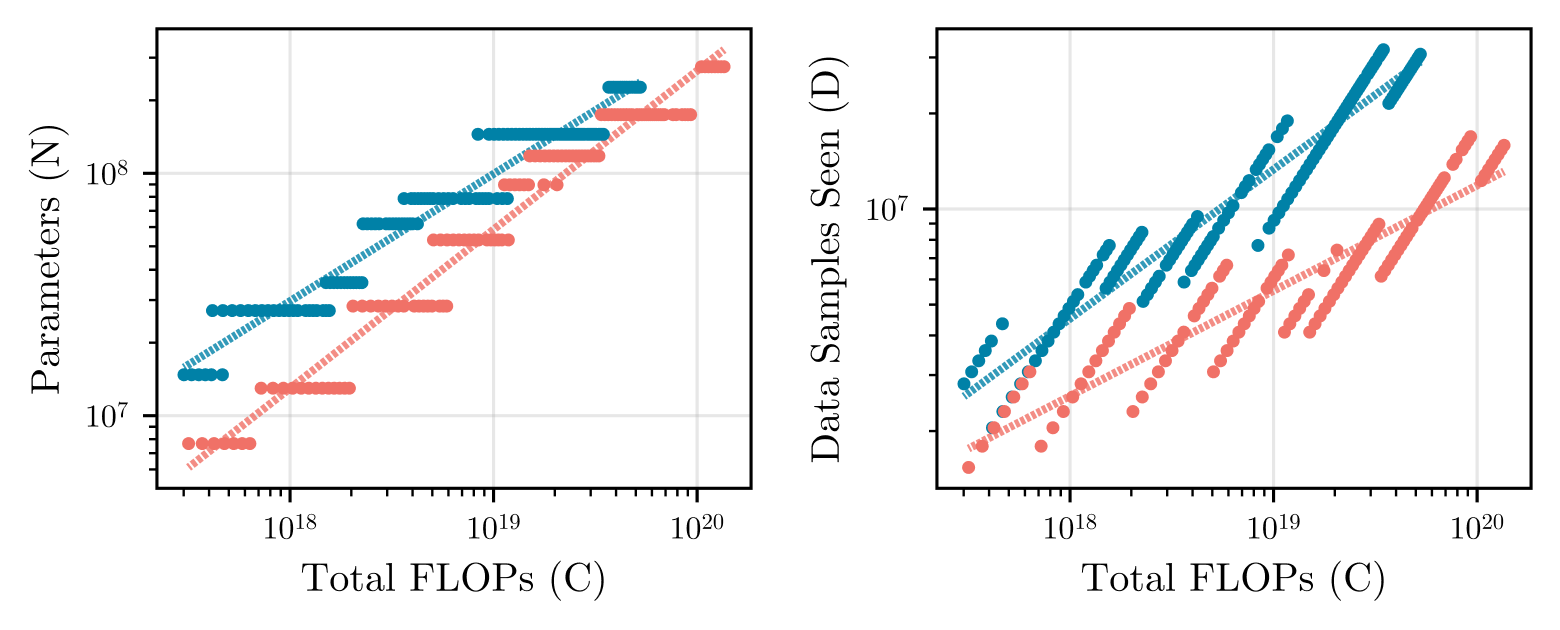
\includegraphics[width=\linewidth]{images/data_param_laws_fix.png}
    \vspace{-0.5cm}
    \caption{
        \textbf{Data and Model Scaling Plots.} 
        While our model~(\textcolor[HTML]{0081A7}{blue}) is optimal when sufficient data is available, decoder-only LVSM~(\textcolor[HTML]{F07167}{red}) performs better with less data. The Pareto frontier analysis shows that our model is more data-hungry. Our model is also less parameter-efficient, although the gap closes as we increase the training compute. However, with sufficient data and compute, our model~(\textcolor[HTML]{0081A7}{blue}) is overall superior in terms of training compute-optimality and rendering speed.
        \vspace{-1\baselineskip}
    }
    \label{fig:opt-model-scaling}
\end{figure}

\paragraph{Scaling Laws.}
We now follow the approach in language modeling~\cite{hoffmann2022training} to answer the question: \textit{for a given compute-budget, what is the optimal performance that can be attained?} For both model families, we sweep across a range of models from around 7M to 300M parameters, training each model for 3-4 different sample counts to densely cover the  FLOP range~\citep{hoffmann2022training}. Our training runs span a compute range of $10^3$ magnitudes: 100 petaflops to 100 exaflops. From this data, we are then able to determine a mapping from compute budgets $C$ to minimum test LPIPs -- the Pareto frontier. 

We plot results in~\figref{fig:two-view-scale}, with their Pareto frontiers marked in dark gray. Plotted on a log-log scale, both models exhibit a consistent downward trend on test LPIPS with more compute. More significantly, the Pareto frontiers of both families have approximately the same slope at points of the same performance (see \suppref{supp:fits}), and SVSM's frontier is shifted left by a factor of $3$. Thus, as an initial result, our scaling laws show us that our encoder-decoder architecture \textit{scales exactly the same as the decoder-only LVSM while using $3\times$ less training-compute.} Qualitative results of this scaling are shown in \figref{fig:qualitative-two-view}, and we see that when FLOP-matched, SVSM has better rendering quality.

\vspace{-1\baselineskip}


\begin{figure*}[t]
    \centering
    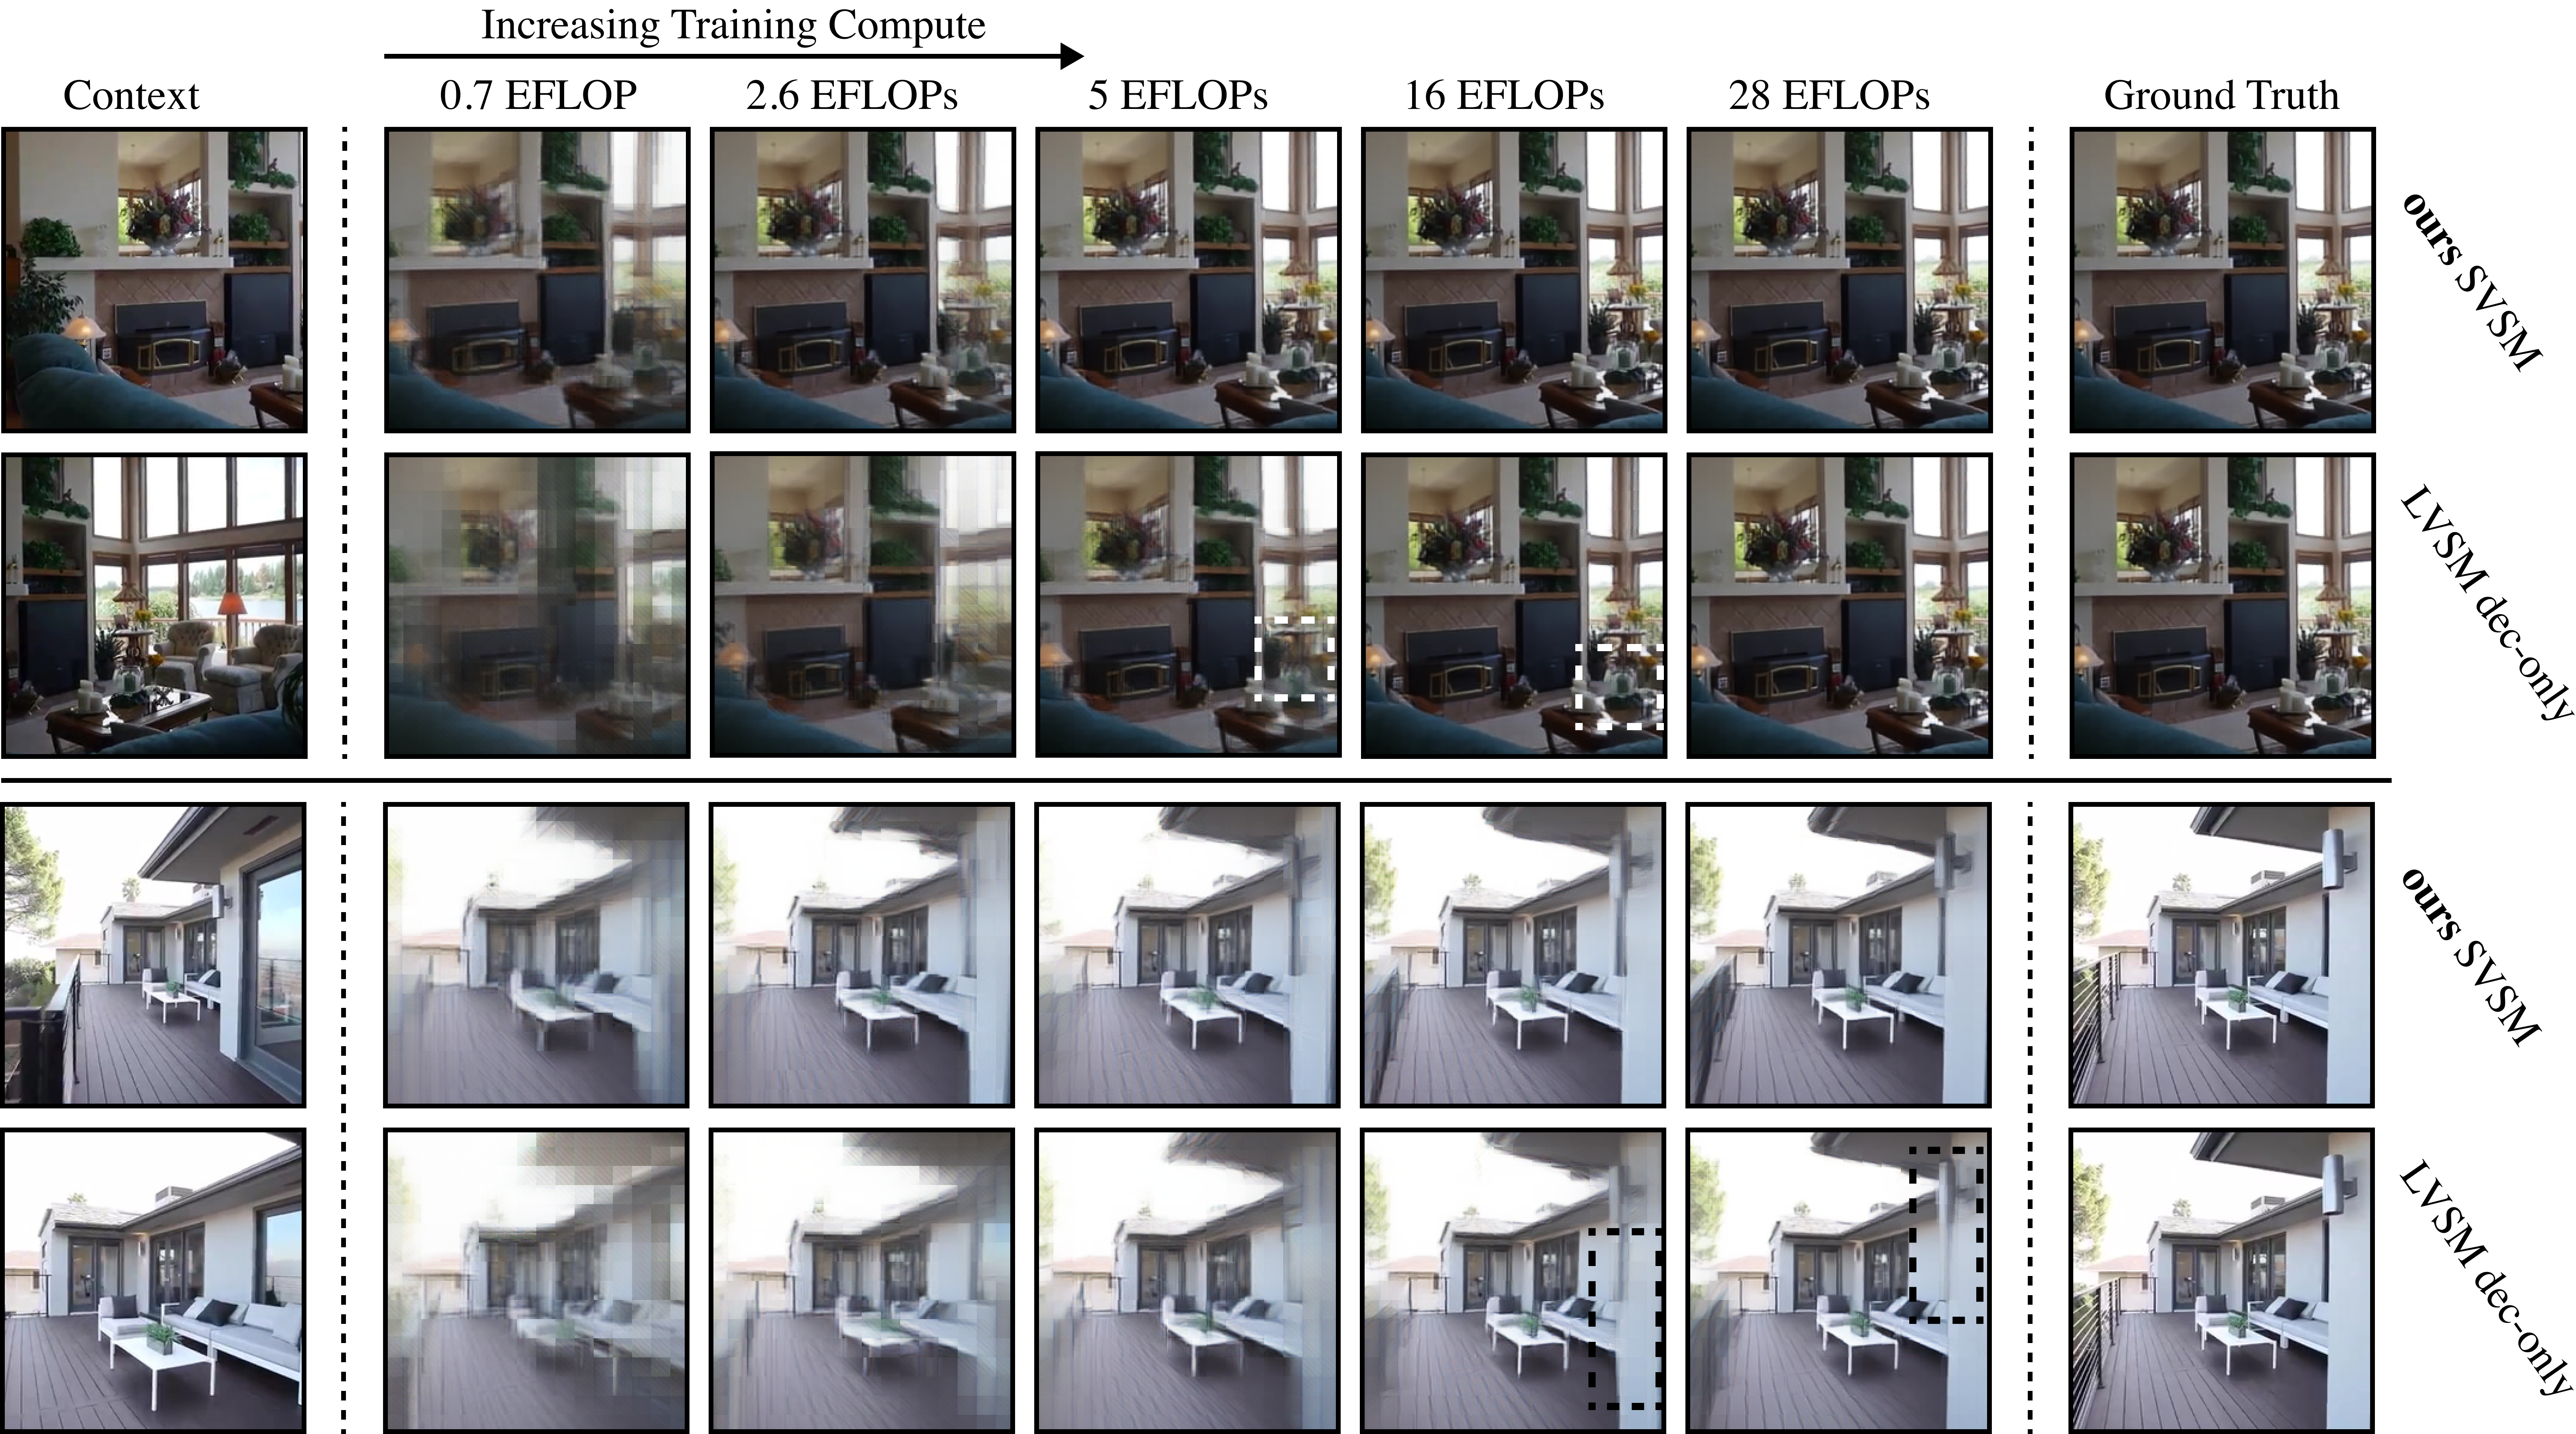
\includegraphics[width=\textwidth]{images/qualitative_twoview_fixed.png}
    \caption{
        \textbf{Qualitative Scaling Behavior}, $V_C = 2$. From left to right, both models steadily increase in rendering quality until reaching near photo-realistic results. Compared vertically, for a given compute-budget, SVSM renderings consistently contain less artifacts.
        \vspace{-1\baselineskip}
    }
    \label{fig:qualitative-two-view}
\end{figure*}
\begin{table}[t]
  \centering
  \begin{threeparttable}
    \scriptsize
    \setlength{\tabcolsep}{3pt} % Kept your spacing

    % Use 'tabular*' to span the full column width
    % 'l' for model names, 'r' for the three da ta columns
    % Added @{\extracolsep{\fill}} to distribute the space
    \begin{tabular*}{\columnwidth}{@{\extracolsep{\fill}} l ccc} 
      \toprule
      
      % --- Supercolumn ---
      & \multicolumn{3}{c}{\textbf{Recon Quality}} \\
      
      % --- Rule for supercolumn ---
      \cmidrule(lr){2-4} 
      
      % --- Subcolumns ---
      \textbf{Model} 
      & \textbf{PSNR} (↑) & \textbf{SSIM} (↑) & \textbf{LPIPS} (↓) \\
      
      \midrule
      
      % --- Data Rows (Filled) ---
      pixelNeRF~\citep{yu2020pixelnerf} & 20.43 & 0.589 & 0.550 \\
      % GPNR~\citep{suhail2022generalizable} & 24.11 & 0.793 & 0.255 \\
      % \citet{du2023learning} & 24.78 & 0.820 & 0.213 \\
      pixelSplat~\citep{charatan2024pixelsplat} & 26.09 & 0.863 & 0.136 \\
      MVSplat~\citep{chen2024mvsplat} & 26.39 & 0.869 & 0.128 \\
      GS-LRM~\citep{zhang2024gs} & 28.10 & 0.892 & 0.114 \\
      % LVSM Enc-Dec~\citep{jin2024lvsm} & 28.58 & 0.893 & 0.114 \\ 
      % LVSM Dec-Only~\citep{jin2024lvsm} & 29.67 & 0.906 & 0.098 \\
      SVSM Enc-Dec \textbf{(ours)} & \textbf{30.01} & \textbf{0.910} & \textbf{0.096} \\
      
      \bottomrule
    \end{tabular*} % <-- Note the 'end' tag is also changed
    
    \caption{
        \textbf{Comparison to Geometry-Aware Methods.}
        Our method achieves a new state-of-the-art on RealEstate10K~\citep{zhou2018stereo} with the set from~\citet{charatan2024pixelsplat}, outperforming not only LVSM, but also prior work with explicit 3D structure. 
        % Our encoder-decoder model, despite having the bottleneck of an intermediate scene representation, outperforms the previous SOTA, LVSM~Dec-Only. Among methods which produce an intermediate scene representation, our method exceeds the previous state-of-the-art, LVSM~Enc-Dec, by a significant margin ($\Delta \text{PSNR}=+1.43$, $\Delta \text{LPIPS}=-0.018$), despite being trained with $1/3$ of the compute.
        % \vspace{-1\baselineskip}
    }
    \label{tab:two_view_STOA}

  \end{threeparttable}
      \vspace{-1\baselineskip}

\end{table}

\paragraph{Optimal Model Choice.}

\begin{table}[h]
\footnotesize
\centering
\begin{tabular}{lcc}
\toprule
\textbf{Model} & Parameter Coeff.\ $a$ & Data Coeff.\ $b$ \\
\midrule
LVSM & 0.65 & 0.33 \\
SVSM & 0.52 & 0.47 \\
\bottomrule
\end{tabular}
\caption{\textbf{Parameter and Data Scaling Coefficients.} As regressed from the plots in \figref{fig:opt-model-scaling}, we find power law coefficients for scaling models and data with respect to compute.
\vspace{-1\baselineskip}
}
\label{tab:opt-model-table}
\end{table}


From our scaling experiments, we can further extract a compute-optimal training recipe for our view synthesis transformers, as demonstrated by~\citet{hoffmann2022training}. For each compute budget $\compute{}$, we determine the corresponding optimal model size $N$ and the amount of training data $D$ used at that point. Then, plotting $N$ and $D$ against $\compute{}$, we can extract the Chinchilla scaling equations (\eqref{eqn:chinchilla}) by fitting lines onto the log-log plots in Fig. \ref{fig:opt-model-scaling}. The recovered coefficients are shown in \tabref{tab:opt-model-table}, which inform how to train models which end on the frontier.

From these results it follows that for SVSM, if we increase our compute budget by a factor of $k\times$, it should approximately be equally allocated between increasing the model size by $\sqrt k$ and increasing data sample count by $\sqrt k$ as $a_{\text{SVSM}} \approx b_{\text{SVSM}}$, matching the findings of the Chinchilla scaling laws~\citep{hoffmann2022training} for language models. For LVSM this relationship does not seem to hold exactly, but the fit still shows that requires significant scaling of data with respect to compute, though to a smaller power. 

\begin{figure*}[t]
    \centering
    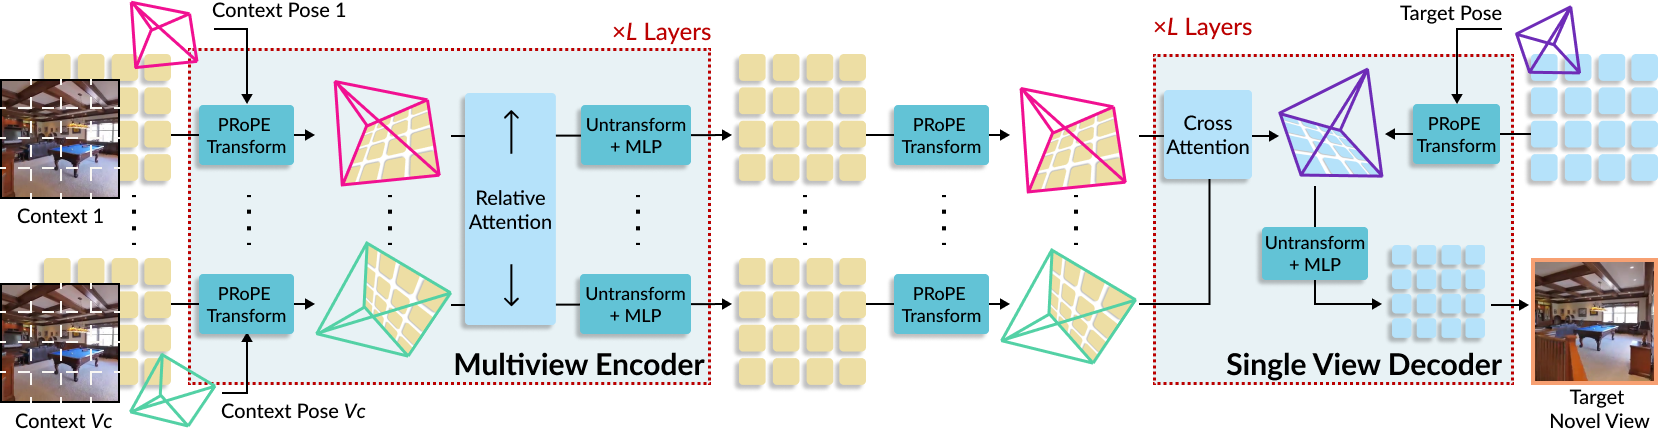
\includegraphics[width=1.0\textwidth]{images/prope_arch.png}
    \caption{\textbf{Multiview PRoPE.} We find that multiview projective RoPE embeddings~\citep{miyato2023gta,kong2024eschernet,li2025cameras} are critical for our model to scale with compute and data in the multiview setting ($V_C>2$). For each layer of the multiview transformer encoder, PRoPE embeddings use context camera poses to transform context view tokens into a common coordinate frames before the attention layer, and apply the inverse transformation before each MLP. To render, both context features and query tokens of the target view are transformed by PRoPE before cross-attention.}
    \vspace{-\baselineskip}
    \label{fig:prope}
\end{figure*}
\begin{figure}
    \centering
    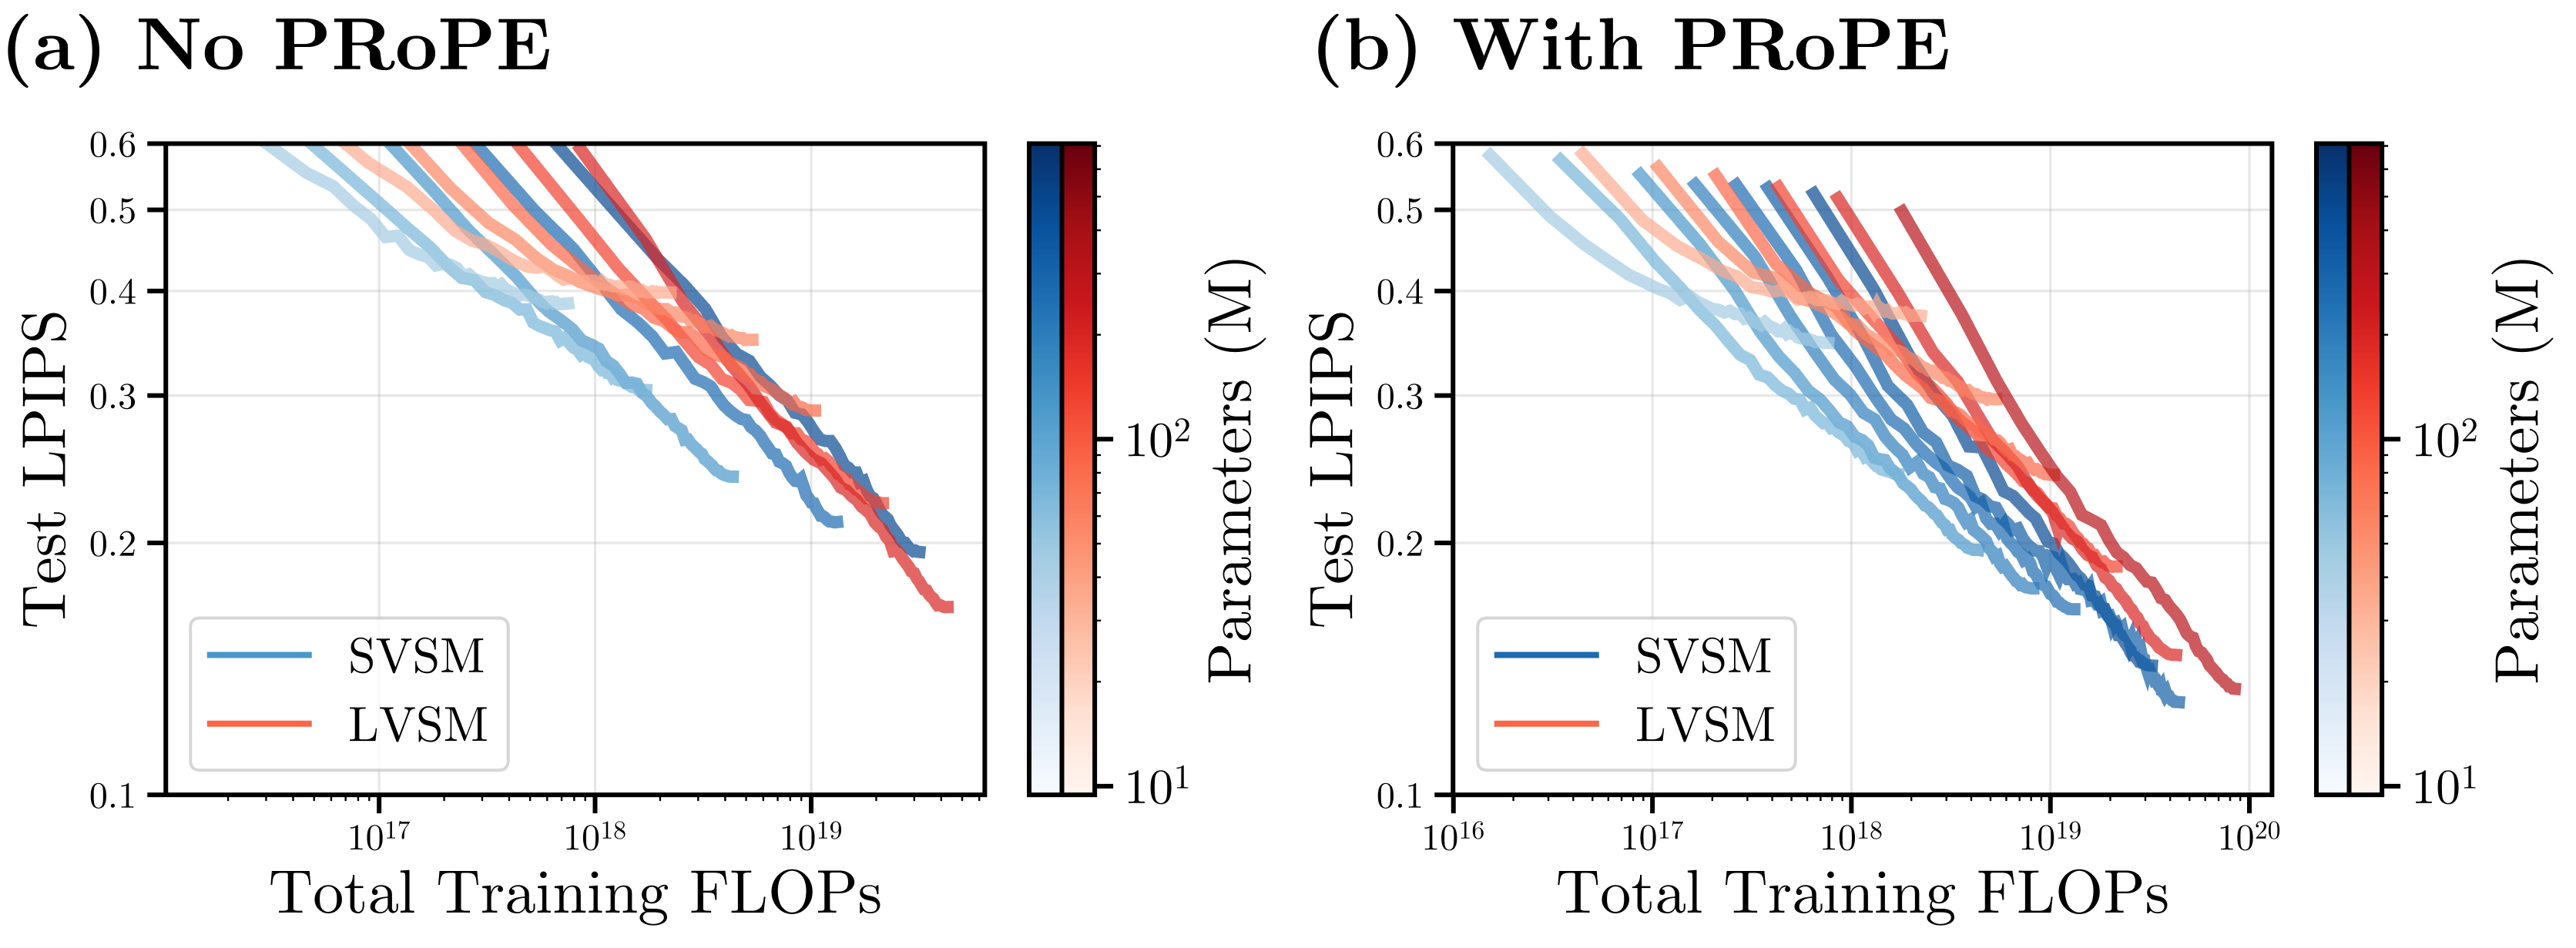
\includegraphics[width=\linewidth]{images/dl3dv_scaling_fixed.png}
    \caption{\textbf{Multiview Scaling Behavior.} Conducted on DL3DV~\cite{ling2024dl3dv}. \textbf{(a)} For $V_C{>}2$, without PRoPE, SVSM saturates and stops scaling much more quickly than LVSM. \textbf{(b)} When PRoPE is added, SVSM continues scaling with a better Pareto-frontier.}
    \label{fig:mv_scale}
\end{figure}

Notably our data sample counts include \emph{repeated scene data}, as we only have access to small, pose-labeled datasets. This differs from standard scaling practice, in which models are typically trained for less than one full epoch~\citep{hoffmann2022training, kaplan2020scaling, zhai2022scaling}. Although we have not yet seen evidence of overfitting in our experiments -- perhaps due to the diversity of view sequences which are sampled during training -- we have shown that increasing scale requires increasing the number data samples. Thus, having access to larger amounts of diverse posed data will be essential for developing large-scale generalizable NVS models.
\vspace{-1\baselineskip}
% Two points of note here:
% \begin{itemize}
%     \item The data quantity analyzed here was analyzed with repeated data -- proper requires more paired data or self-supervised NVS
%     \item \textbf{Reference appendix for increased scene quantity giving better test loss.}
% \end{itemize}





% [maybe more discussion here?]



% To answer this question, for both families of models, we train 



% \begin{itemize}
%     \item We sweep across a range of models and data samples (details in appendix)
%     \item We plot LPIPs loss against FLOPs
%     \item In linear regions, same slope, but different intercept
%     \item Compute vs. Data and Compute vs. Model size scaling laws
%     \item Maybe make a statement about data diversity in NVS
% \end{itemize}



% \subsection{Scaling laws for model and data, $C > 2$}


% \begin{itemize}
%     \item PRoPE ?
%     \item need experiments without PRoPE -- done.
%     \item need prettier plots for the scaling laws in this case .... 
% \end{itemize}


% \vspace{-1\baselineskip}
\paragraph{SVSM-420M/740M Results.}
%
\looseness=-1
Finally, combining our scaling law findings, we train two separate models --- SVSM-420M and SVSM-740M, aptly named to denote their parameter counts --- to compare against the original results of LVSM's largest model on RealEstate10K. Due to compute-constraints, we train our models at a lower total budget of around $10^{21}$ FLOPs and a batch size of $256$,  approximately half the FLOPs and exactly half the batch size used by LVSM.  We train two models under this budget: (1) a flop-matched model with the 24 layer LVSM model for a forward pass of a single training sample with $V_C = 2, V_T=  6$ and; (2) A model whose parameter count is given by plugging the budget\footnote{To be more specific, we plug $\compute/4$ into the scaling law, in order to adjust for the scaling law being derived off of $16\times 16$ patch experiments, while this final budget is under $8\times 8$ patches, which requires roughly $4\times$ as much compute.} $\compute$ and the coefficients from \tabref{tab:opt-model-table} to \eqref{eqn:chinchilla}.

While we train with under half the compute, our scaling laws in Sec.~\ref{subsec:scalinglaws} predict equal performance with three times less compute. Thus, as predicted by our scaling laws and validated empirically by the results in \ref{tab:two-view-result} both SVSM models outperform decoder-only LVSM. Notably, SVSM-420M, the model trained in accordance with our scaling laws performs the best. For completeness, we also show reported results from prior work on this benchmark in \tabref{tab:two_view_STOA}. 

Furthermore, we also benchmark the \textit{rendering speed}, which is calculated with $V_T = 1$ to simulate real-time online rendering with respect to a stream of input poses. Additional details can be found in \suppref{supp:rendering}. As seen in \tabref{tab:two-view-result}, SVSM generally renders much faster than decoder-only LVSM, and  is eclipsed only once $V_C$ increases to $8$. 

%While the gap is marginal $\approx 0.3$ PSNR, it was achieved with 45\% of the compute, and half the batch size. If batch size 512 was used, we expect that the gap would be much larger.

% \textbf{Rendering speed.} Thus far, we have only discussed training FLOPs. Now, with our final models, we benchmark rendering speed. All rendering speeds are calculated with $V_T = 1$ to simulate real-time, online rendering with respect to a stream of input poses. 





